\section{The communicating stationary region and a maximal hypersurface}
\label{st:section}

Throughout this section the hypotheses of the connected, nondegenerate
equality case hold.  We use the fields furnished by
Propositions~\ref{va:stationary-data} and~\ref{va:boundary}.  Put
\[
 \mathfrak R=\mathbb R_z\times\operatorname{int}\Omega,
 \qquad \xi=\partial_z,
 \qquad W=u^2-|X|_g^2.
\]
Thus
\begin{equation}\label{st:product}
 \mathbf G=-u^2dz^2+g_{ij}(dx^i+X^i dz)(dx^j+X^j dz)
          =-Wdz^2+2X^\flat dz+g.
\end{equation}
Here and below products of one-forms in metric formulas are symmetric
products; in particular, $dU\,dV$ has components
$G_{UV}=G_{VU}=1/2$.  The smooth two-form $\mathbf F$ and the metric
are invariant under the complete flow of $\xi$.  The vector $\xi$ is
future causal and nonzero on $\mathfrak R$, since $u>0$ there and
$u\geq |X|_g$.  Also
\begin{equation}\label{st:original-time}
 \mathbf G^{-1}(dz,dz)=-u^{-2}<0.
\end{equation}
Consequently $z$ is a temporal function even where $W=0$.  Near infinity
and on a deleted collar of $S$ we have $W>0$, and the equations there
are the source-free Einstein--Maxwell equations.  The constant
$\kappa>0$ is the one in Proposition~\ref{va:boundary}.

\subsection{Communication with the end}

On the original stationary end chart, write $\rho=|x|$ for the
Euclidean spatial radius.

\begin{proposition}\label{st:communication}
Let $\mathfrak E=\mathbb R\times\{\rho>R\}$, with $R$ sufficiently
large.  Taking chronological past and future within $\mathfrak R$, one has
\[
 I^-(\mathfrak E)=\mathfrak R=I^+(\mathfrak E).
\]
\end{proposition}

\begin{proof}
Write $\mathfrak A=I^-(\mathfrak E)$; the future case has the same proof
with time orientation reversed.  The end has timelike Killing orbits,
so $\mathfrak E\subset\mathfrak A$.  The set $\mathfrak A$ is open and
invariant under every Killing translation.  It is connected: a point of
$\mathfrak A$ can be joined to $\mathfrak E$ by a timelike curve entirely
in $\mathfrak A$, and $\mathfrak E$ is connected.  Hence
$\mathfrak A=\mathbb R\times A$ for a connected open subset $A$ of
$\operatorname{int}\Omega$ containing its distant end.

Suppose that its relative boundary $\mathfrak H=\partial_{\mathfrak R}
\mathfrak A$ is nonempty.  A boundary of a chronological past is
achronal and locally separates its past side from an excluded future
side.  To recall the local regularity used here, choose a small coordinate
cylinder whose vertical lines are timelike.  Achronicity permits at most
one boundary point on each such line.  The openness of the past set and
local timelike cone bounds show that the boundary is a graph over a
spatial ball, with a uniform Lipschitz bound.  Shrinking the cylinder
removes any edge of this graph.  This description also shows that both
of its local sides are nonempty.

The boundary is invariant.  At every differentiability point its tangent
hyperplane therefore contains $\xi$.  An achronal tangent hyperplane
cannot contain a timelike vector.  Since $\xi$ is nonzero and causal,
it is null there, and the hyperplane is precisely $\xi^\perp$.
Continuity gives $W=0$ throughout $\mathfrak H$.  This proves smoothness
as well.  Indeed, in the preceding graph chart write the graph as
$x^0=f(x^1,x^2,x^3)$.  The smooth plane field $\xi^\perp$ is transverse
to the vertical direction.  Its graph slopes are smooth functions
$a_i(x^0,x)$; the weak derivatives of $f$ satisfy
$\partial_i f=a_i(f(x),x)$ almost everywhere.  The right sides are
continuous.  Mollification, or integration on coordinate lines, shows
that these are the classical derivatives of a $C^1$ function.  This
identity then gives successively $C^2,C^3,\ldots$ regularity.  In
particular no regular-level-set assumption on $W$ is involved.

Intersecting with $z=0$ gives a smooth embedded two-sided surface
$C=\partial A$ in $\operatorname{int}\Omega$.  The intersection is
transverse because the $z$-slice is spacelike while the null normal
$\xi$ is nonzero.  Invariance identifies $\mathfrak H$ with
$\mathbb R\times C$.  Since $W>0$ in a deleted collar of $S$ and on
the end, $C$ lies in a compact subset of $\operatorname{int}\Omega$.
It is closed there and thus compact.  A compact smooth embedded
surface has finitely many components: finitely many connected local
submanifold charts cover it, and each component contains one of these
charts.  In particular there is no accumulating family of extra
frontier components.

Choose the normal $\nu_C$ into the end-side exterior.  On each connected
component of $C$,
\[
 \xi=u(n+\varepsilon\nu_C),\qquad \varepsilon\in\{1,-1\},
\]
where $n$ is the future normal to $z=0$ and the sign is constant on that
component.  The null second form of $\mathfrak H$ along its Killing
normal is zero: for tangent vectors $Y,Z$ to a spacelike section it is
symmetric by hypersurface orthogonality and has symmetric part
$\tfrac12(\mathcal L_\xi\mathbf G)(Y,Z)=0$.  Its trace therefore
vanishes.  Thus $C$ is marginal for one of the two expansion signs on
each component.

The connected collar of the connected surface $S$ contains no frontier
point.  It is consequently wholly contained in $A$ or wholly excluded
from $A$.  The closure of $A$ in $\Omega$ is a connected closed smooth
exterior with full boundary $C\cup S$ in the first case and $C$ in
the second.  It contains the distant end.  The local excluded side at
every point of $C$ shows that its complementary obstacle contains an
additional nonempty open subset outside the original obstacle.  Its
components have the marginal signs just determined, together with the
original sign on $S$ if that component is present.  This contradicts
Proposition~\ref{va:enlarged-obstacle}.  Hence $\mathfrak H$ is empty.
Connectedness of $\mathfrak R$ proves the assertion.
\end{proof}

The componentwise choice of sign in
Proposition~\ref{va:enlarged-obstacle} is essential here: a boundary of
a chronological future need not have the future marginal sign of the
original surface.

\subsection{A smooth bifurcation attachment}

We first prove the regularity fact needed when the stationary lapse
vanishes at the original boundary.  All covariant derivatives in the
next lemma are spacetime covariant derivatives taken on the open
collar.  Their limiting coefficients are evaluated in a spatial
orthonormal frame and the future normal of the original slices.

\begin{lemma}\label{st:covariant-jets}
Suppose $u|_S=0$.  The tensors
$\boldsymbol\nabla^j\mathbf F$ and
$\boldsymbol\nabla^j\mathbf{Rm}$, for every integer $j\geq0$, have
smooth one-sided limiting coefficients at $S$ in this frame.  So does
$\boldsymbol\nabla\xi$.  At $S$ the latter tensor is the endomorphism
$B$ given by
\begin{equation}\label{st:boost-generator}
 B\nu=\kappa n,\qquad Bn=\kappa\nu,
 \qquad B|_{TS}=0.
\end{equation}
Every limiting curvature and Maxwell jet is invariant under $B$, acting
on all its tensor and derivative slots.  It is also invariant under
the map $I_b$ which reverses both $n$ and $\nu$ and fixes $TS$.
\end{lemma}

\begin{proof}
Choose a smooth spatial orthonormal frame $e_i$ on an original collar
patch and extend it, and $n$, by stationarity.  For spatial directions
the spacetime connection is nonsingular:
\[
 \boldsymbol\nabla_{e_i}n=K_i{}^j e_j,
 \qquad
 \boldsymbol\nabla_{e_i}e_j=\Gamma_{ij}^k e_k+K_{ij}n.
\]
In particular spatial covariant differentiation preserves smooth
one-sided coefficients.  The spatial derivatives of $\xi=u n+X$ are
\begin{equation}\label{st:derivative-killing}
 \boldsymbol\nabla_{e_i}\xi
 =(e_i u+K(e_i,X))n
   +(uK_i{}^j+D_iX^j)e_j.
\end{equation}
Skew symmetry of $\boldsymbol\nabla\xi$ determines its remaining
components without division by $u$.  The boundary identities
$u=0$, $X=0$, $DX=0$, and $du=\kappa\nu^\flat$ give
Equation~\eqref{st:boost-generator}.  Also
$[\xi,e_i]=[\xi,n]=0$, so the connection coefficients along $\xi$
are the coefficients of $\boldsymbol\nabla_{e_i}\xi$ and
$\boldsymbol\nabla_n\xi$ and are bounded and smooth in the same
sense.

The order-zero Maxwell coefficients are the original electric and
magnetic fields.  Gauss--Codazzi determines
$\mathbf R_{ijkl}$ and $\mathbf R_{nijk}$ from $g,K$ and their
spatial derivatives.  In the deleted collar the Ricci tensor is
\[
 \mathbf{Ric}_{ab}
 =2\left(\mathbf F_{ac}\mathbf F_b{}^c
       -\tfrac14\mathbf G_{ab}\mathbf F_{cd}\mathbf F^{cd}\right),
\]
because the Maxwell stress is trace free.  The contraction identity
\begin{equation}\label{st:ricci-block}
 \mathbf R_{ninj}=\sum_k\mathbf R_{kikj}-\mathbf{Ric}_{ij}
\end{equation}
then supplies the remaining curvature block (with the same curvature
convention in Gauss--Codazzi and this identity).  All order-zero
coefficients therefore have smooth limits.

Here is an induction which controls every normal derivative.  Write
$F_j=\boldsymbol\nabla^j\mathbf F$ and
$R_j=\boldsymbol\nabla^j\mathbf{Rm}$, with derivative slots listed
from outermost to innermost.  Suppose all orders below $j$ have smooth
limits.  Any component of order $j$ having a spatial derivative slot
has a smooth limit: commute that derivative to the outermost slot and
use the displayed spatial connection formulas.  The commutators are
sums of contractions of lower derivatives of curvature with lower
derivatives of the tensor being differentiated.  Their total derivative
order is $j-2$, so the induction hypothesis controls every term.

It remains to treat derivative slots $n,\ldots,n$.  Apply $j-1$
covariant derivatives to closure and co-closure of $\mathbf F$, and
evaluate their free derivative slots on $n$.  Metric compatibility
allows these tensor identities to be contracted directly; derivatives
of a chosen extension of the frame do not enter.  For spatial $i,l$
they read
\begin{align}
 F_j(n^j;i,l)
 &=-F_j(n^{j-1},i;l,n)-F_j(n^{j-1},l;n,i),\label{st:maxwell-curl-jets}\\
 F_j(n^j;n,i)
 &=\sum_lF_j(n^{j-1},l;l,i).\label{st:maxwell-div-jets}
\end{align}
Here $n^j$ means $j$ derivative slots equal to $n$.  Every right-hand
side has a spatial derivative slot and was already controlled.  These
identities give all of $F_j$ first.

The differentiated differential Bianchi identity similarly gives
\begin{equation}\label{st:bianchi-jets}
 R_j(n^j;i,l,a,b)
 =-R_j(n^{j-1},i;l,n,a,b)
  -R_j(n^{j-1},l;n,i,a,b).
\end{equation}
By pair symmetry this covers every curvature component except the
block with two normal tensor slots, $R_j(n^j;n,i,n,l)$.
Differentiating
Equation~\eqref{st:ricci-block} supplies that component.  The
differentiated Ricci tensor is a sum of products of the already
controlled $F_0,\ldots,F_j$.  This closes the joint induction.  Each
right-hand side has smooth coefficients on the original closed
collar, so the conclusion is smooth one-sided dependence, including
all spatial derivatives, rather than merely bounded limits.  No
identity in the induction solves a time evolution equation by
dividing by $u$.

For $T=\boldsymbol\nabla^j\mathbf F$ or
$\boldsymbol\nabla^j\mathbf{Rm}$, Killing invariance of the
connection gives $\mathcal L_\xi T=0$.  Written covariantly this is
\[
 0=\boldsymbol\nabla_\xi T+(\boldsymbol\nabla\xi)\cdot T.
\]
The first term tends to zero: it is
$u\boldsymbol\nabla_nT+X^i\boldsymbol\nabla_{e_i}T$, and the
next-order jets have just been controlled.  Thus $B\cdot T=0$ at
the edge.  In the null basis $n+\nu,n-\nu$ the two eigenvalues of
$B$ are $\kappa,-\kappa$.  A component of an invariant covariant
tensor can be nonzero only when its total boost weight is zero.
Counting its derivative slots as well as its tensor slots, it
therefore contains equal numbers of the two normal null directions.
Their simultaneous sign reversal has even total degree.  This proves
the $I_b$ invariance.
\end{proof}

\begin{lemma}\label{st:smooth-parity}
Let $a(r,y)$ be smooth for $r\geq0$, with $y$ in a compact smooth
manifold.  If all odd $r$-derivatives vanish at $r=0$, then
$a(r,y)=a_0(r^2,y)$ for a function $a_0$ smooth up to $r^2=0$.
If all even derivatives vanish, then
$a(r,y)=r a_1(r^2,y)$ with $a_1$ smooth.  Both assertions hold for
tensor coefficients in smooth local frames and uniformly with all
tangential derivatives.
\end{lemma}

\begin{proof}
In the first case Taylor's formula to arbitrarily high order gives
\[
 a(r,y)=\sum_{j=0}^{L}a_j(y)r^{2j}
                  +r^{2L+2}b_L(r,y),
\]
where $b_L$ is smooth.  Put $p=r^2$.  Repeatedly applying
$\partial_p=(2r)^{-1}\partial_r$ to the remainder, up to order
$h\leq L$, bounds the result by $C p^{L+1-h}$; the same estimate
holds after any prescribed tangential derivatives.  Hence
$a(\sqrt p,y)$ has the derivatives at $p=0$ prescribed by the
polynomial, continuously to every order.  In the second case,
Hadamard's formula writes $a=r b$ with $b$ smooth; the Taylor
coefficients of $b$ have the parity of the first case.  This proof
also treats a smooth flat remainder and makes no analyticity
assumption.
\end{proof}

\begin{proposition}\label{st:attachment}
There is a smooth time-oriented Lorentzian manifold
$(\widetilde{\mathfrak R},\mathbf G)$ containing $\mathfrak R$ and a
compact smooth spacelike surface $B_0$ naturally identified with $S$,
such that the following properties hold.
\begin{enumerate}
\item The Killing field extends smoothly, has complete flow, vanishes
on $B_0$, and is a nondegenerate boost in its normal plane with
constant $\kappa$.
\item The two-form $\mathbf F$ has a smooth invariant extension.
The field equations continue to hold on the original right wedge.
\item A neighborhood of the added surfaces is a band
$\{|UV|<p_0\}\times S$, with
\[
 \xi=\kappa(V\partial_V-U\partial_U),\qquad
 B_0=\{U=V=0\},
\]
and its overlap with $\mathfrak R$ is $U,V>0$.
\item If $u|_S>0$, the original stationary chart extends to the
future horizon $U=0,V>0$, with each original boundary section at a
finite positive $V$.  If $u|_S=0$, the original slice extends to $B_0$.
In both cases the metric of $B_0$ is the original metric on $S$.
\end{enumerate}
\end{proposition}

\begin{proof}
First suppose $u|_S>0$.  The equation
$dW=2\kappa X^\flat$ on $S$ makes $W$ a global positive defining
function on a boundary collar.  Use coordinates $(W,y)$ there.
Division of a smooth tensor vanishing on the boundary by its defining
function gives a smooth one-form $\beta$ with
\[
 X^\flat=\frac{dW}{2\kappa}+W\beta.
\]
Set
\begin{equation}\label{st:positive-coordinates}
 V=e^{\kappa z},\qquad U=W e^{-\kappa z},\qquad p=UV=W.
\end{equation}
Substitution into Equation~\eqref{st:product} cancels the singular
terms and gives
\begin{equation}\label{st:positive-extension}
 \mathbf G=\kappa^{-2}dU\,dV+\frac{2}{\kappa}U\beta\,dV+g,
\end{equation}
where $\beta,g$ are pulled back from $(p,y)$; in such pullbacks
$dW=VdU+UdV$.  This is smooth at both null faces and at their
intersection.  At the intersection its normal block is
$\kappa^{-2}dU\,dV$ and its tangential block is $g|_{TS}$.

To extend the Maxwell tensor, write in the original regular chart
\[
 \mathbf F=dz\wedge e+\alpha_2,
 \qquad e=\iota_\xi\mathbf F.
\]
At $W=0$ the vector $\xi$ is the null normal of a smooth Killing
horizon.  Its null second form vanishes by the Killing equation.
The null Raychaudhuri equation, either with an affine generator or
with its nonaffine term proportional to the zero expansion, gives
$\mathbf{Ric}(\xi,\xi)=0$.  Electrovacuum holds up to this horizon
by continuity from the deleted collar.  Thus
\[
 0=\mathbf{Ric}(\xi,\xi)
    =2|\iota_\xi\mathbf F|_{\mathbf G}^2.
\]
The one-form $\iota_\xi\mathbf F$ annihilates $\xi$.  On the
orthogonal space of a null vector the metric is positive semidefinite
with precisely its null line as kernel.  The last equality therefore
implies that $e$ is proportional to the metric dual of $\xi$, hence
to $dW$, at the horizon.  Smooth division gives
$e=b\,dW+W\gamma$ with $b,\gamma$ smooth on the collar.  The
potentially singular terms become
\[
 dz\wedge b\,dW=-\frac{b}{\kappa}dU\wedge dV,
 \qquad dz\wedge W\gamma=\frac{U}{\kappa}dV\wedge\gamma.
\]
All remaining terms are smooth pullbacks from $(p,y)$.

Now suppose $u|_S=0$.  In original normal distance $s$ the boundary
identities give $u=\kappa s+O(s^2)$ and $X=O(s^2)$ with smooth
Taylor factors.  Thus the tensors
\begin{equation}\label{st:orbit-collar}
 A_s=W^{-1}X^\flat,\qquad
 h_s=g+W^{-1}X^\flat\otimes X^\flat
\end{equation}
are smooth up to $S$, and $h_s$ is positive definite and equals $g$
there.  The metric is
$\mathbf G=-W(dz-A_s)^2+h_s$.  Let $(r,y)$ be the Gaussian normal
coordinates of $h_s$ at $S$, and put
\[
 H(r,y)=\int_0^r(A_s)_r(t,y)\,dt,
 \qquad z'=z-H(r,y).
\]
In these coordinates $A_s-dH$ has no radial component.  It follows
that $G_{rr}=1$ and $G_{ra}=0$ for $a\ne r$.  Therefore the curves
$r\mapsto(z',r,y)$ are unit spacelike geodesics, and
$Y_A=\partial_{y^A}$ and $\xi=\partial_{z'}$ along them are
Jacobi fields.  Notice that $r$ is a smooth original defining
function with $r=s+O(s^2)$.

We prove the precise parity of their coefficients.  The connection
along these geodesics is smooth one-sided: their velocities are
smooth linear combinations of original spatial directions and
$\xi$, whose connection coefficients were controlled in
Lemma~\ref{st:covariant-jets}.  A parallel orthonormal frame with a
prescribed limiting basis at $r=0$ is therefore obtained by a linear
ODE with smooth coefficients on a closed half interval.  The radial
velocity has limiting value $\nu$.  The values $Y_A(0)$ are tangent
to $S$, while $\xi(0)=0$ and
$D_r\xi(0)=\kappa n$.

For completeness, $D_rY_A(0)$ is normal to $S$.  The Killing identity
$\boldsymbol\nabla(\boldsymbol\nabla\xi)=\mathbf{Rm}*\xi$
shows that the tangential derivative of $B=\boldsymbol\nabla\xi$
vanishes at the edge.  Hence the projector
$P=B^2/\kappa^2$ onto $\operatorname{span}(n,\nu)$ is parallel
there in every tangent direction.  The vector $(1-P)\partial_r$
vanishes at the edge, with its tangential derivatives.  Differentiating
this equality tangentially yields
$(1-P)\boldsymbol\nabla_{Y_A}\partial_r=0$.  Since coordinate
fields commute, this is the assertion about $D_rY_A(0)$.

Let $I_b$ act in the parallel frame as in
Lemma~\ref{st:covariant-jets}.  The $j$th radial derivative of
curvature at zero is its $j$th covariant derivative contracted with
$j$ copies of $\nu$.  Its transformation under $I_b$ consequently
acquires the factor $(-1)^j$.  Differentiate the Jacobi equation
\[
 D_r^2Y+\mathbf R(Y,\partial_r)\partial_r=0.
\]
The initial values are fixed by $I_b$ and their initial derivatives
change sign.  Induction in this equation gives
$I_b D_r^jY(0)=(-1)^jD_r^jY(0)$ for both $Y=Y_A$ and $Y=\xi$.
The contractions $\mathbf G(Y_A,Y_B)$,
$\mathbf G(\xi,Y_A)$ and $\mathbf G(\xi,\xi)$ therefore have
only even Taylor coefficients.  The initial values and
Equation~\eqref{st:boost-generator} give
\[
 \mathbf G(\xi,Y_A)=O(r^2),\qquad
 \mathbf G(\xi,\xi)=-\kappa^2r^2+O(r^4).
\]
For $\mathbf F$, the same differentiated contraction rule uses all
its covariant jets.  Contractions on two Jacobi fields have even
parity, and contractions with one radial velocity and one Jacobi
field have odd parity.  Also $\mathbf F(\xi,Y_A)=O(r^2)$ because
$\xi(0)=0$.  Lemma~\ref{st:smooth-parity} now gives the following
actual smooth coefficient formulas, with $p=r^2$:
\begin{align}
 \mathbf G={}&dr^2+(-\kappa^2p+p^2a)\,dz'^2
       +2p b_A\,dz' dy^A+c_{AB}\,dy^A dy^B,\label{st:even-metric}\\
 \mathbf F={}&\tfrac12 f_{AB}\,dy^A\wedge dy^B
       +p e_A\,dz'\wedge dy^A+r q_A\,dr\wedge dy^A
       +r d\,dr\wedge dz'.\label{st:even-maxwell}
\end{align}
All coefficients in these displays are smooth in $(p,y)$ up to
$p=0$.  Smooth dependence of the geodesic and parallel-frame ODEs
on $y$ makes these conclusions uniform with every tangential
derivative.  The statements are tensorial on overlapping charts of
$S$, so they define global tensors on its collar.

Set
\begin{equation}\label{st:zero-coordinates}
 V=r e^{\kappa z'},\qquad U=r e^{-\kappa z'}.
\end{equation}
Then
\[
 dr^2-\kappa^2r^2dz'^2=dU\,dV,
 \qquad
 p\,dz'=\frac{U\,dV-V\,dU}{2\kappa},
\]
\[
 r\,dr=\frac{V\,dU+U\,dV}{2},
 \qquad r\,dr\wedge dz'=\frac{dU\wedge dV}{2\kappa}.
\]
Equations~\eqref{st:even-metric}--\eqref{st:even-maxwell} are thus
smooth in $(U,V,y)$.  Their metric at $U=V=0$ has normal block
$dU\,dV$ and tangential block $g|_{TS}$.

In each case extend the finitely many smooth coefficient tensors in
$p\geq0$ to $|p|<p_0$, keeping the displayed invariant forms.
A smooth extension exists by collar extension in each coordinate
patch and a partition of unity on the compact $S$.  Lorentz signature
and time orientation hold near $B_0$ by the nondegenerate leading
blocks.  They hold on the entire sufficiently small band: the boost
$U\mapsto e^{-\kappa t}U$, $V\mapsto e^{\kappa t}V$ takes any
point with $p\ne0$ to one with $|U|=|V|=\sqrt{|p|}$, and takes a
point on a punctured null face arbitrarily close to $B_0$.  The
extended formulas are invariant under these boosts.

Glue this open band to the deleted collar of $\mathfrak R$ by
Equation~\eqref{st:positive-coordinates} or
Equation~\eqref{st:zero-coordinates}.  This is a collar gluing of
smooth manifolds.  To check its separation property, a sequence in
the overlap which tends to an added null face has $p\to0$ or
unbounded original time and cannot have a limit in $\mathfrak R$;
a sequence tending to the outer collar boundary has no limit in the
open added band.  No pair of distinct retained points is therefore
identified by a limiting overlap sequence.  Local collar charts and
the old charts give a Hausdorff, second-countable manifold.  The
translations and boosts agree on the overlap, and both are defined
for every real parameter.  Their resulting Killing flow is complete.

In the positive-lapse case the original regular chart gives
$U=0,V=e^{\kappa z}$ on $S$; in the zero-lapse case $r=0$ gives
$B_0$ and the original $z=0$ slice has a smooth finite $z'$ offset.
These observations also identify the induced metric on $B_0$ and
the indicated original boundary.  The extension was constructed
for this geometric purpose; only its restriction to $\mathfrak R$
is used in the field equations below.
\end{proof}

\begin{remark}\label{st:orbit-boundary}
The tensors in Equation~\eqref{st:orbit-collar} will also be useful
after obtaining staticity.  In the positive-lapse case they satisfy
\[
 A_s=\frac{1}{2\kappa}d\log W+\beta,
 \qquad
 h_s=g+\frac{dW^2}{4\kappa^2W}
       +\frac{1}{\kappa}dW\,\beta+W\beta^2.
\]
Thus $h_s$ extends as a smooth positive tensor to the collar with
defining function $r=\sqrt W$, and is invariant under $r\mapsto-r$
as a tensor.  Its coefficients with one radial index have odd
parity; the others have even parity.  In the zero-lapse case $A_s$
is smooth in the original structure, and $\sqrt W$ is a smooth
positive multiple of the original defining function.  The two
smooth collar structures need not coincide in the positive-lapse
case.
\end{remark}

\subsection{The stationary end and a global temporal graph}

\begin{proposition}\label{st:stationary-end}
The stationary end admits coordinates $(t,x^1,x^2,x^3)$ with
$\xi=\partial_t$.  Writing $\rho=|x|$ in this chart, one has for
every fixed integer $j\geq0$
\begin{equation}\label{st:strong-end}
 \mathbf G_{ab}-\eta_{ab}=O_j(\rho^{-1}),\qquad
 \mathbf F_{ab}=O_j(\rho^{-2}).
\end{equation}
All these estimates have the corresponding scaled H\"older bounds.
The coordinates are obtained from a constant rest chart by stationary
corrections $O_{2,\gamma}(\rho^{1-q_1})$, where
$1/2<q_1<q_0<\min(q,1)$ and $0<\gamma<1$ can be chosen smaller
as needed.  In particular, on the end the orbit metric $h_s$ satisfies
$h_s-\delta=O_j(\rho^{-1})$ and $W=1+O_j(\rho^{-1})$.
\end{proposition}

\begin{proof}
Proposition~\ref{va:stationary-data} gives a constant limiting metric
for Equation~\eqref{st:product}, with error $O_2(\rho^{-q_0})$,
and a unit timelike limiting $\xi$, since
$(b^0)^2-|b|^2=1$.  A constant linear change of coordinates puts this
metric in rest form $\eta$ while keeping the new spatial coordinates
constant along Killing orbits.  Explicitly, in the limiting product
coordinates one can take $t_*=z-b_i x^i$ and a spatial linear map
whose Euclidean quadratic form is $\delta_{ij}+b_i b_j$.  The old
and new spatial radii are comparable.  Maxwell components remain
$O_1(\rho^{-2})$ under this constant change.

We describe the coordinate improvement to account for the weak initial
derivative bounds.  For a stationary scalar the wave operator has the
form
\[
 L=\mathbf G^{ij}\partial_i\partial_j+d^i\partial_i,
 \qquad
 \mathbf G^{ij}=\delta^{ij}+O_1(\rho^{-q_0}),\quad
 d^i=O_0(\rho^{-1-q_0}).
\]
It is uniformly elliptic on a sufficiently distant end because $W>0$
there.  Solve $L\chi^a=-\boldsymbol\Box x_*^a$, for the three
linear spatial rest coordinates and for $x_*^0=t_*$.  The sources
are $O_{0,\gamma}(\rho^{-1-q_1})$; this H\"older estimate follows
on scaled annuli from the available second metric derivatives, after
decreasing $q_1$ and, if necessary, $\gamma$.

Here is a construction of the right inverse at this weight.  Extend
the scalar operator to the Euclidean Laplacian inside a large sphere
with a smooth cutoff.  This extension is only for the coordinate
equation.  For a source $f=O_{0,\gamma}(\rho^{-1-q_1})$ the Newton
kernel with its constant term subtracted on the far tail defines
\[
 P f(x)=-\frac1{4\pi}\int_{\mathbb R^3}
 \left(\frac1{|x-y|}-\frac{\chi_\infty(y)}{|y|}\right)f(y)\,dy,
\]
where $\chi_\infty=1$ outside a fixed ball and vanishes near zero.
The tail is absolutely convergent because the difference of kernels
is $O(|x|\,|y|^{-2})$.  Splitting the integral into
$|y|<|x|/2$, $|y|\asymp |x|$, and $|y|>2|x|$ gives
$|Pf(x)|\leq C(1+|x|)^{1-q_1}$.  For example, the last region is
bounded by
$C|x|\int_{2|x|}^{\infty}s^{-1-q_1}\,ds$; the other regions
give the same power.  Differentiation of the kernel for first
derivatives and scaled interior Schauder estimates for second
derivatives give the weighted $C^{2,\gamma}$ bound.  Thus $P$ is a
bounded right inverse from weight $-1-q_1$ to weight $1-q_1$.

After rescaling the cutoff radius to one, the coefficient norm of
$L-\Delta$ between these spaces tends to zero with that radius.
The convergent Neumann series for $1+P(L-\Delta)$ gives the required
corrections $\chi^a=O_{2,\gamma}(\rho^{1-q_1})$.  They are smooth
by local elliptic regularity.  Their first derivatives tend to zero,
so the new spatial coordinates are a diffeomorphism on a further
tail.  Since the corrections are stationary,
\[
 \boldsymbol\Box t=\boldsymbol\Box x^i=0,
 \qquad \xi(t)=1,\qquad \xi(x^i)=0.
\]
In particular $\xi$ remains exactly $\partial_t$.

In these harmonic coordinates the reduced Ricci equation has scalar
principal part
\begin{equation}\label{st:harmonic-equation}
 \mathbf G^{ij}\partial_i\partial_j\mathbf G_{ab}
   =\mathcal Q_{ab}(\mathbf G,\partial\mathbf G)
       -2\mathbf{Ric}_{ab},
\end{equation}
where $\mathcal Q$ is quadratic in first derivatives with smooth
bounded coefficients near $\eta$.  The coordinate construction
starts with scaled $C^{1,\gamma}$ bounds for the metric error and
scaled $C^{0,\gamma}$ bounds for the Maxwell field.  The Ricci source
is quadratic in $\mathbf F$, since the end is electrovacuum.
Schauder estimates in Equation~\eqref{st:harmonic-equation} therefore
give scaled $C^{2,\gamma}$ bounds for the metric.  The Maxwell
equations then give one additional field derivative.  One way to
see the latter step precisely is to square closure and co-closure:
\[
 \boldsymbol\Box\mathbf F=\mathbf{Rm}*\mathbf F.
\]
By stationarity this is elliptic.  Its coefficients have the metric
regularity just obtained and its zeroth-order source has scaled
$C^{0,\gamma}$ bounds.  Interior $W^{2,p}$ estimates first improve
the bounded first field derivatives to $C^{0,\gamma'}$ bounds for
any fixed $\gamma'<1$ by taking $p$ large; Schauder estimates then
apply.  Equivalently the stationary Hodge system is elliptic because
the symbol of $d+\delta$ squares to
$\mathbf G^{ij}\zeta_i\zeta_j>0$ for a nonzero spatial covector.
Repeating these two estimates gives, on every scaled annulus,
\[
 \partial^j(\mathbf G-\eta)=O(\rho^{-q_1-j}),\qquad
 \partial^j\mathbf F=O(\rho^{-2-j})
\]
for every fixed $j$.  The constants may depend on $j$.  This
bootstrap uses only the original two metric derivatives and one
field derivative to start, and only ellipticity on the distant
timelike region.

It follows from Equation~\eqref{st:harmonic-equation}, replacing its
principal coefficients by $\delta^{ij}$ and using the just-proved
second derivative estimate, that
\begin{equation}\label{st:integrable-laplacian}
 \Delta_\delta(\mathbf G_{ab}-\eta_{ab})
       =O_j(\rho^{-2-2q_1}+\rho^{-4})
\end{equation}
for every $j$.  The right side is integrable in three dimensions
because $2q_1>1$.  Multiply a component of the decaying perturbation
by a cutoff on the end and call its Euclidean Laplacian $f$.  The
unsubtracted Newton integral of $f$ is now $O(\rho^{-1})$: the
inner region is bounded by $C\rho^{-1}\|f\|_{L^1}$ and the
comparable and outer regions are $O(\rho^{-2q_1})$.  Its difference
from the cutoff perturbation is an entire harmonic function tending
to zero, hence vanishes by the maximum principle.  Scaled estimates
for the Poisson equation and its derivatives prove the first
estimate in Equation~\eqref{st:strong-end} to every order.  The
field estimate is already known.  One further derivative implies
each desired scaled H\"older estimate.  Finally
$h_{s,ij}=\mathbf G_{ij}-\mathbf G_{0i}\mathbf G_{0j}/\mathbf G_{00}$
and $W=-\mathbf G_{00}$ give the asserted orbit estimates.
\end{proof}

\begin{lemma}\label{st:temporal-graph}
There is a smooth function $s_0$ on $\mathfrak R$ satisfying
$\xi(s_0)=1$, whose differential is timelike, such that
\begin{equation}\label{st:time-near-bifurcation}
 s_0=\frac{1}{2\kappa}\log\frac VU
\end{equation}
near the attachment and $s_0=t+\mathrm{constant}$ on the harmonic
rest end of Proposition~\ref{st:stationary-end}.  Each level of $s_0$ is
a Cauchy hypersurface of $\mathfrak R$.
\end{lemma}

\begin{proof}
The covector in Equation~\eqref{st:time-near-bifurcation} is
timelike on a sufficiently small positive collar.  This can be
checked at $U=V=\sqrt p$ in the smooth metrics of
Proposition~\ref{st:attachment} and then everywhere on the positive
collar by boost invariance.  In the positive-lapse case it is
$dz-(2\kappa W)^{-1}dW$.  Choose a smooth radial cutoff $\chi(W)$
equal to one near zero and zero outside this collar and set
\[
 s_0=z-\frac1{2\kappa}\int^W\frac{\chi(w)}{w}\,dw.
\]
The integration constant is chosen so that the displayed local
formula holds exactly.  Its differential is a convex combination
of $dz$ and $dz-(2\kappa W)^{-1}dW$.  Both covectors have value
one on the future causal $\xi$, so they lie in the same component
of the timelike covector cone; that cone is convex.  This proves
timelikeness and extends $s_0$ to $z$ plus a constant off the collar.

In the zero-lapse case Equation~\eqref{st:time-near-bifurcation}
is $z'=z-H(r,y)$.  Cut off $H$ in a sufficiently thin original
collar.  The additional spatial differential stays bounded because
$H=O(r)$ and a cutoff derivative of order $r^{-1}$ is multiplied
by $H$.  For any bounded spatial one-form $\lambda$,
\[
 \mathbf G^{-1}(dz+\lambda,dz+\lambda)
 =|\lambda|_g^2-u^{-2}(1-\lambda(X))^2.
\]
Here $u=\kappa r+O(r^2)$ and $X=O(r^2)$.  Thus the negative term
dominates uniformly on a sufficiently thin collar, including the
cutoff annulus.  This again continues the desired time as $z$ plus
a constant.

On the far end replace this time by the harmonic rest time $t$
plus a constant.  Both time covectors have value one on $\xi$;
their limiting Minkowski covectors, and the segment joining them,
are uniformly timelike.  Their difference of functions is a spatial
linear function plus $O(\rho^{1-q_1})$ and a constant.  If the
interpolation cutoff varies by one over a sufficiently long interval
of $\log\rho$, the extra differential is at most $C/L$, where
$L$ is the length of that interval.  Choose $L$ large, and then its
starting radius large.  This error is smaller than the uniform
timelike margin of the convex segment.  The resulting smooth
function has all the asserted local formulas and is temporal
globally.  Each modification was a globally defined stationary
function, so $\xi(s_0)=1$ is preserved.

We check the Cauchy assertion quantitatively.  Write
$r=\sqrt{UV}$ in the positive collar and use $(s_0,r,y)$ there.
At $s_0=0$ the smooth extension has a positive radial coefficient,
a positive tangential metric, and time coefficient a negative
constant times $r^2$.  The remaining terms in the formulas of
Proposition~\ref{st:attachment} can be absorbed into these leading
quadratic forms for small $r$.  Uniformly for a causal tangent
vector one obtains
\begin{equation}\label{st:collar-cone}
 |dr|^2+|dy|^2\leq C r^2|ds_0|^2.
\end{equation}
Here $|dy|$ is measured in a fixed metric on the compact $S$.
Boost invariance extends the bound to every $s_0$.  In particular
$|d\log(UV)/ds_0|\leq C$, so a causal curve cannot reach the
deleted inner end in a finite amount of $s_0$ time.  On the outer
end, Equation~\eqref{st:strong-end} gives
$|dx/ds_0|\leq C$, excluding escape to spatial infinity in finite
time.  On the compact part between these two regions, temporality
and stationary smooth coefficients give the same bounded-speed
estimate in any fixed auxiliary spatial metric.  This argument
also covers compact loci where $W=0$, since $u$ and $ds_0$ remain
nondegenerate there.

If an inextendible future causal curve had a finite upper endpoint
for its $s_0$ range, these estimates would confine it to a compact
spatial set away from both ends and make its spatial coordinates
Cauchy as $s_0$ approaches that endpoint.  It would have a limit
in $\mathfrak R$ and could be extended by a short timelike curve,
a contradiction.  The past argument is identical.  Thus its
$s_0$ range is all of $\mathbb R$, and strict monotonicity gives
exactly one intersection with every level.
\end{proof}

\subsection{Causality of the attachment and its domain of dependence}

Let
\begin{equation}\label{st:sigma-definition}
 \Sigma=\{s_0=0\}\cup B_0\subset\widetilde{\mathfrak R}.
\end{equation}
Near $B_0$ it is parametrized by $U=V=r\geq0$ and $y\in S$.
It is therefore a smooth spacelike hypersurface with boundary $B_0$.
It is closed: the local parametrization includes its only limits on
the added faces, while escaping the asymptotically Euclidean end
has no limit in the spacetime.  It is connected and has a compact
core and one Euclidean end.  Its induced metric is complete with
the boundary included.

\begin{lemma}\label{st:attachment-causality}
After decreasing the width of the added band, the full spacetime
$\widetilde{\mathfrak R}$ is strongly causal and $\Sigma$ is acausal.
Moreover
\begin{equation}\label{st:domain-equality}
 \operatorname{int}D_{\widetilde{\mathfrak R}}(\Sigma)=\mathfrak R.
\end{equation}
The equality holds using either inextendible causal curves or the
timelike-curve convention for domains of dependence.
\end{lemma}

\begin{proof}
We retain only a sufficiently small open band $|UV|<p_0$ on the
added side.  The invariant smooth metric formulas imply
\[
 \mathbf G^{UU}=U^2a(p,y),\quad
 \mathbf G^{VV}=V^2b(p,y),\quad
 \mathbf G^{UV}=c(p,y),\qquad c\geq c_0>0,
\]
where $a,b,c$ are smooth and bounded for $|p|<p_0$.  Choose a fixed
large $C$ and define
\begin{equation}\label{st:corrected-null-coordinates}
 \mathcal U=U e^{-Cp},\qquad \mathcal V=V e^{-Cp}.
\end{equation}
A direct computation gives
\begin{equation}\label{st:corrected-gradient}
 e^{2Cp}|d\mathcal U|_{\mathbf G}^2
 =U^2\{a(1-Cp)^2-2C(1-Cp)c+C^2p^2b\}.
\end{equation}
The analogous formula interchanges $U,a$ with $V,b$.  Taking $C$
large and then $p_0$ small makes the braces strictly negative.
The two gradients are nonzero even on their respective null faces.
With the right-wedge future orientation,
$\mathcal U$ is nonincreasing and $\mathcal V$ nondecreasing
along future causal curves in the band.  Their difference
$\mathcal T=\mathcal V-\mathcal U$ has timelike differential:
the two causal covectors have opposite orientations and are
linearly independent.  In particular $\mathcal T$ is temporal
through the intersection of the faces.

These monotonicities also control curves which leave a coordinate
neighborhood.  First the right wedge is causally convex in the full
attachment.  A future curve leaving it across a null face must cross
$U=0$ into $U\leq0,V>0$.  It cannot return across that face because
$\mathcal U$ cannot increase to positive values.  It cannot leave
the added band elsewhere except through the right wedge, the only
old region continuing beyond the band.  The corresponding past
statement uses $V=0$.  The same sign argument excludes a departure
and return through the right wedge for endpoints in any one of the
other open quadrants.  Thus the temporal functions $s_0$ and
$\mathcal T$ establish strong causality at points off the faces.

There is one additional global issue at a face: a curve could
otherwise travel far into the right wedge and return near that
face.  Fix a small $p_1>0$ at which the exact logarithmic formula
\eqref{st:time-near-bifurcation} still holds.  Suppose a future
causal curve with endpoints $a,b$ sufficiently close to a face
leaves $p<p_1$ through $e$, and subsequently returns through $f$.
Both crossing points have $p=p_1$ in the right wedge.  The segment
between them has nondecreasing $s_0$, by causal convexity and
Lemma~\ref{st:temporal-graph}.  Hence
\[
 \frac{V_f}{U_f}\geq\frac{V_e}{U_e},\qquad
 V_f\geq V_e,\quad U_f\leq U_e.
\]
Monotonicity on the initial and final band segments then gives
\begin{equation}\label{st:no-return}
 \mathcal U(a)\mathcal V(b)
 \geq \mathcal U(e)\mathcal V(f)
 \geq p_1 e^{-2Cp_1}>0.
\end{equation}
If either factor has the wrong sign, such a curve is already
impossible.  Otherwise the left side tends to zero as both endpoints
approach any fixed point on a null face, contradicting the fixed
positive lower bound.  This excludes the excursion.

For a curve that stays in the band, both corrected coordinates stay
between their endpoint values.  The map
$(U,V)\mapsto(\mathcal U,\mathcal V)$ is a local diffeomorphism
throughout the smaller band, since its Jacobian is
$e^{-2Cp}(1-2Cp)>0$.  Thus endpoints near a fixed face point confine
$U,V$ to a fixed small coordinate box.  In that box and for all
$y\in S$, compactness and the timelike covector $d\mathcal T$
give a uniform causal speed bound
$|dy|\leq C\,d\mathcal T$.  A sufficiently small difference of
endpoint $\mathcal T$ values prevents angular escape from any
prescribed neighborhood of the point.  Combined with
Equation~\eqref{st:no-return}, this is the defining local
no-departure-and-return property of strong causality at every face
point, including $B_0$.

The open part of $\Sigma$ is acausal by its temporal level-set
description and causal convexity of the right wedge.  No causal
curve can join it to $B_0$.  A future curve from $B_0$ starts with
$\mathcal U\leq0,\mathcal V\geq0$ and cannot enter the right
wedge; a past curve has the opposite obstruction from
$\mathcal V\leq0$.  A hypothetical connection in the other
direction is the same statement with endpoints reversed.  A causal
curve between two points of $B_0$ would have both corrected
coordinates constant zero.  It would then be tangent to $B_0$,
whose metric is positive definite, and must be constant.  Hence
the closed hypersurface $\Sigma$ is acausal.

Every inextendible causal curve in the full spacetime through a
point of the right wedge has a maximal portion in that wedge which
is inextendible as a curve of the wedge.  By
Lemma~\ref{st:temporal-graph} this portion intersects $s_0=0$.
Thus $\mathfrak R\subset D(\Sigma)$, and openness gives the
inclusion into its interior.

For the reverse inclusion, in the left wedge $U,V<0$ the complete
Killing orbits are timelike and avoid $\Sigma$.  In the future
quadrant $U<0,V>0$, a timelike curve can be continued to the past
into the left wedge while staying in the band.  To verify this
directly, boost a point to $(U,V)=(-d,d)$, where
$d=\sqrt{|UV|}$.  At fixed $y$ follow the past-directed segment
\[
 U(\lambda)=-d+\tfrac12d\lambda,
 \qquad V(\lambda)=d-2d\lambda,
 \qquad 0\leq\lambda\leq1.
\]
Its leading normal metric norm is a strictly negative constant
times $d^2$, and the perturbation is smaller uniformly when the
band is small.  It is therefore timelike.  Along it
$|UV|\leq d^2<p_0$, and it ends in the left wedge.  Continue there
on a complete timelike Killing orbit in the past direction; in
the future direction remain in the future quadrant until an
inextendible end of the curve.  Both portions avoid $\Sigma$.
The past quadrant has the time-reversed construction.  Corners can
be rounded inside the open timelike cones.  Thus every point of
the three other open quadrants lies on an inextendible timelike
curve avoiding $\Sigma$.  None belongs to $D(\Sigma)$ even for
the timelike-curve convention.  Finally each null face has empty
interior and borders an excluded quadrant.  It cannot contribute
to $\operatorname{int}D(\Sigma)$.  This proves
Equation~\eqref{st:domain-equality} with either convention.
\end{proof}

\begin{figure}[tbp]
 \centering
 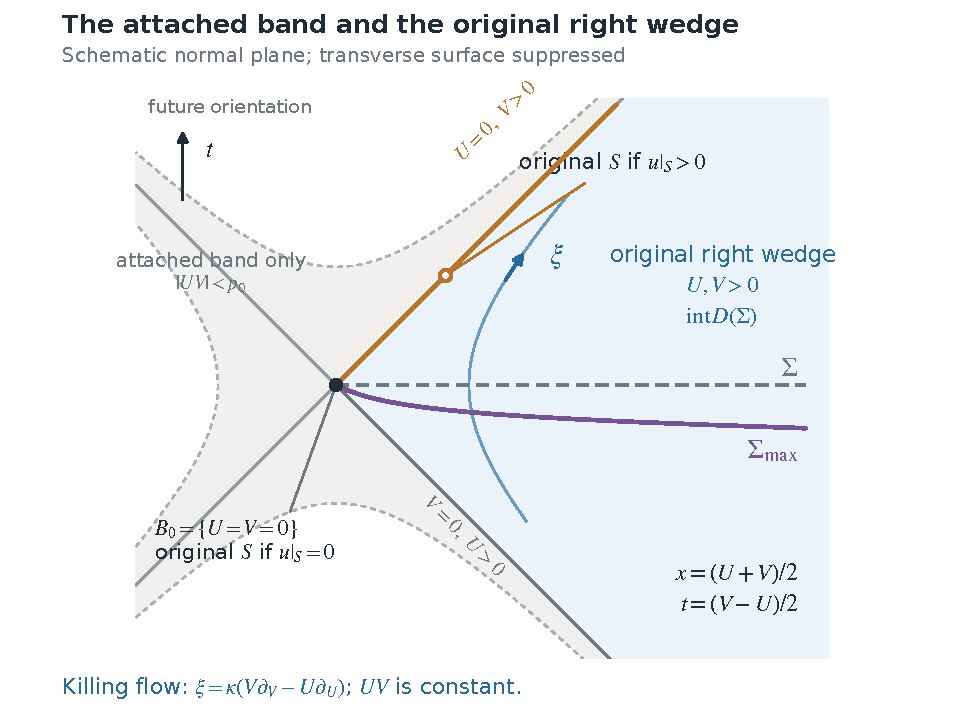
\includegraphics[width=\linewidth]{figures/bifurcation-attachment.pdf}
 \caption{Normal-plane schematic of the bifurcation attachment, with
 $x=(U+V)/2$, $t=(V-U)/2$, and the transverse compact surface suppressed.
 The original right wedge $U,V>0$ is $\operatorname{int}D(\Sigma)$;
 only the band $|UV|<p_0$ is adjoined in the remaining quadrants.
 The auxiliary slice $\Sigma$ and the maximal slice $\widehat\Sigma$
 (denoted $\Sigma_{\rm max}$ in the figure and $\Sigma'$ in
 Section~\ref{ri:section}) end at the same bifurcation surface $B_0$.
 The original boundary $S$ lies at $B_0$ when $u|_S=0$, and
 on the future horizon $U=0$, $V>0$ when $u|_S>0$.
 The curved arrow denotes Killing flow.  Slice shapes are schematic,
 with $\Sigma$ equal to $t=0$ near the attachment; the drawing is
 not an exact conformal diagram.}
 \label{fig:st-attachment}
\end{figure}

\subsection{Application of the maximal-hypersurface theorem}

\begin{proposition}\label{st:maximal-slice}
Fix $q_2\in(1/2,1)$.  There exists a smooth spacelike maximal hypersurface
$\widehat\Sigma\subset\widetilde{\mathfrak R}$ with
$\partial\widehat\Sigma=B_0$, whose interior is Cauchy in
$\mathfrak R$.  Every complete Killing orbit of $\mathfrak R$
meets it exactly once.  In the harmonic rest chart of
Proposition~\ref{st:stationary-end} its end is a graph $t=f(x)$ satisfying
\begin{equation}\label{st:maximal-decay}
 f=O(\rho^{1-q_2}),\qquad
 \partial f=O(\rho^{-q_2}),\qquad
 \partial^2 f=O(\rho^{-1-q_2}).
\end{equation}
The graph has the corresponding higher differentiability and scaled
H\"older estimates.  Its Killing translates cover the right wedge.
\end{proposition}

\begin{proof}
We apply the class-(b) existence theorem of Chru\'sciel and Wald
\cite[Definitions 2.1, 2.3 and 2.4, Equation (4.1),
Theorem 4.2]{ChruscielWald1994}.  We verify its geometric conditions
on the particular spacetime just constructed.

The spacetime is smooth, time oriented and strongly causal by
Proposition~\ref{st:attachment} and
Lemma~\ref{st:attachment-causality}.  The hypersurface $\Sigma$
in Equation~\eqref{st:sigma-definition} is connected, closed,
acausal, spacelike and smooth up to the compact boundary $B_0$.
It is the union of a compact core and one Euclidean end.  The
smooth Killing field has a complete flow on the full spacetime
and fixes $B_0$ pointwise.  The end lies in a stationary chart with
uniformly negative $G_{00}$, uniformly positive spatial metric,
and $\xi=\partial_t$.  Equation~\eqref{st:strong-end} supplies
all derivatives and the weighted H\"older bounds of their
asymptotic definition.  In particular we may use differentiability
order two and the fixed exponent $q_2\in(1/2,1)$.

Let $\mathfrak M_{\rm ext}$ denote the Killing development of
this end, as in their definition of black and white hole regions.
It is exactly a stationary end of the original right wedge.
Equation~\eqref{st:domain-equality} identifies the open domain of
dependence as $\mathfrak R$, and
Proposition~\ref{st:communication} gives
\[
 \mathfrak R\subset I^-(\mathfrak M_{\rm ext})
                  \cap I^+(\mathfrak M_{\rm ext}).
\]
Thus neither black nor white hole points meet that open domain;
this is their Equation (4.1).  All hypotheses of
\cite[Theorem~4.2]{ChruscielWald1994} are now satisfied.
We record the analytic details that give regularity at the fixed
boundary and the derivative estimates in this application.  Let
$\tau_0$ be the smooth time function furnished by
\cite[Proposition~4.2]{ChruscielWald1994}, and let
$\Sigma_* = \{\tau_0=0\}\cap D(\Sigma)$ be its zero hypersurface
in the closed domain, with boundary $B_0$.  Its interior is Cauchy
in $\mathfrak R$.  On the end $\tau_0$ is Killing time; choose
the additive constant of the harmonic rest coordinate so that
$\tau_0=t$ there.  On this strong end we first make the reference
graph maximal outside a compact set.  Here is a direct construction.  Rescale a
sufficiently distant end by $x=R y$, $t=R\theta$, and extend its
stationary metric coefficients to Minkowski coefficients inside
$|y|=1$.  The extended coefficients satisfy
\[
 \partial^j(\mathbf G-\eta)
   =O(\varepsilon\langle y\rangle^{-1-j}),\qquad
 \varepsilon=O(R^{-1}),\qquad \langle y\rangle=1+|y|,
\]
with the same scaled H\"older bounds.  This auxiliary extension is
used only to solve the end graph equation.  For a stationary graph
$\theta=a(y)$ its normalized maximal equation is
$\Delta a+\mathcal Q(a)=0$.  It depends on $Da,D^2a$, not on $a$.
Use the norm controlling
\[
 \frac{|a|}{\log(2+|y|)},\qquad
 \langle y\rangle|Da|,\qquad
 \langle y\rangle^2|D^2a|
\]
and the corresponding scaled H\"older seminorm, with $a(0)=0$.
The Euclidean Newton operator with its constant tail subtracted,
followed by subtraction of its value at zero, is a bounded right
inverse from $C^{0,\gamma}_{-2}$ to this space.  Indeed, splitting
the integral into $|z|<|y|/2$, $|z|\asymp|y|$, and
$|z|>2|y|$ gives the logarithmic bound for its value and
$O(\langle y\rangle^{-1})$ for its first derivative; local scaled
Schauder estimates give the second derivative and its seminorm.
The subtracted kernel is $O(|y||z|^{-2})$ in the last region,
so that integral converges absolutely.

On a ball of radius $C\varepsilon$ in this norm,
$\mathcal Q(0)=O_{0,\gamma}(\varepsilon\langle y\rangle^{-2})$
and the Lipschitz norm of $\mathcal Q$ into
$C^{0,\gamma}_{-2}$ is $O(\varepsilon)$.  These estimates follow
by writing the principal coefficients as their Euclidean values
plus $O(\mathbf G-\eta)+O(|Da|^2)$; all remaining terms contain
a metric derivative.  The contraction map $a\mapsto-P\mathcal Q(a)$
therefore gives the required graph.  Differentiating its uniformly
elliptic equation on scaled annuli gives all higher derivatives.
Returning to $x$ and cutting off the graph on a fixed annulus gives
a smooth spacelike reference hypersurface $\Sigma_e$ equal to
$\Sigma_*$ on the compact core, and maximal on the distant end, where its
height $a_e$ satisfies
\[
 a_e=O(\log\rho),\qquad \partial^j a_e=O(\rho^{-j})
 \quad(j\geq1).
\]
The cutoff is spacelike because its gradient is small on that
annulus.  The end Killing time $\tau_e=t-a_e$ still has
$\mathbf G-\eta=O_j(\rho^{-1})$ in its coordinates.

Subtract the same cut-off end correction from $\tau_0$ and
call the resulting time function $\tau$.  Its differential remains
timelike: it is unchanged on the compact core, and the correction
has uniformly small gradient in the transition annulus and the
end.  Thus $\tau$ is smooth through $B_0$, has $\Sigma_e$ as
its zero hypersurface in $D(\Sigma)$, and equals $\tau_e$ on the distant end.
Its zero level is Cauchy in $\mathfrak R$: the compact and inner
ends are unchanged, and the end correction is sublinear with
vanishing derivative, so the end causal speed bound and no-escape
argument, or \cite[Lemma~4.2]{ChruscielWald1994}, apply.
Exhaust $\Sigma_e$ by its
compact truncations, whose boundaries are $B_0\cup C_i$ with
$C_i$ an end coordinate sphere.  Compactness of their domains of
dependence is supplied by
\cite[Theorem~3.2]{ChruscielWald1994}, using the communication
condition already verified.  It is this compactness, not merely
compactness of the truncations, that permits the smooth Dirichlet
construction of \cite[Theorem~4.2]{Bartnik1984}.  As in the cited
proof, its domain and edge conditions hold for these acausal
truncations.  We obtain smooth maximal spans $M_i$ with the exact
boundary $B_0\cup C_i$.

For clarity, the uniform height argument permits this fixed inner
boundary.  Choose a fixed sufficiently distant cylinder
$\rho=R_0$, and translate $M_i$ by a Killing parameter $b_i$ so
that its least $\tau$ value on the cylinder is $1$.
Spacelikeness bounds the oscillation on that cylinder uniformly.
The compactness statement
\cite[Corollary~3.6]{ChruscielWald1994} then confines the translated
compact portions to one compact set.  The geometric constants in
Bartnik's tilt estimates are uniform on these surfaces: on the
compact portion this follows from the smooth regular time $\tau$,
and on the end from its stationary identification with $\tau_e$
and the strong coefficient bounds.  In particular the curvature,
the lapse and its first logarithmic derivative, and the derivative
of the reference unit normal are bounded.  If $b_i\leq0$, the translated
outer boundary has time $b_i$, while $B_0$ is fixed and has time
zero.  Comparison on the end with the maximal reference translates
also bounds the translated height above: its interface height is
bounded, and its outer height is nonpositive.  Together with the
compact-core bound this gives a uniform upper bound for the
translated height.  Thus the cylinder is separated by at least one
unit of time from both boundary values, and its distance below
the supremum of the translated height is uniformly bounded.
The interior tilt estimate
\cite[Theorem~3.1(iv), Equation~(3.14)]{Bartnik1984}
gives a uniform tilt bound there.  The exterior test-function
argument in \cite[proof of Theorem~5.3, Equations~(5.13)--(5.18)]{Bartnik1984}
now bounds $-b_i$.  That argument integrates only over the end,
after subtracting an exterior barrier and the outer boundary time.
Its cylinder trace has bounded oscillation and bounded tilt; these
are precisely the two inner-boundary estimates used in its boundary
term.  The fixed surface $B_0$ is outside this integration region
and contributes no additional term.  The test function gives
$\log(2+|b_i|)\leq C$, with $C$ independent of $i$.
For large positive $b_i$, an additional bounded translation puts
the greatest cylinder time at $-1$; applying the same argument with
time reversed bounds $b_i$.  This is the translation argument in
\cite[proof of Theorem~4.2, Equations~(4.22)--(4.26)]{ChruscielWald1994}.
Consequently $|b_i|$ is uniformly bounded.  Compactness on the
interior and comparison with the maximal reference translates on
the end give $|\tau|\leq C$ on the original $M_i$.

The ensuing tilt estimate includes the actual boundary.  Both
components of $\partial M_i$ lie in $\{\tau=0\}$; their ambient
mean-curvature vectors have a uniform bound, since $B_0$ is fixed
and smooth and $C_i$ are end spheres.  The boundary maximum
argument in \cite[Theorem~3.1(iii), Equations~(3.10)--(3.12)]{Bartnik1984}
therefore gives a uniform tilt bound on all of $M_i$, including
$B_0$.  Its hypotheses bound the geometry of the prescribed edge;
they do not assume the unknown boundary gradient.  In smooth
coordinates across $B_0$ this makes the graph equation uniformly
elliptic with fixed smooth boundary data.  Boundary gradient
H\"older estimates and Schauder estimates, followed by
bootstrapping, give uniform bounds of every order on each fixed
closed collar.  The interior estimates give the same conclusion
on every compact subset.  A diagonal subsequence consequently
converges smoothly, up to the same embedded $B_0$, to a spacelike
maximal hypersurface.

One can also read off its end estimates directly.  Relative to
$\Sigma_e$, the graphs $M_i$ have uniformly bounded heights.
For any fixed $0<\beta<1$, the graphs
$a_e\pm C\rho^{-\beta}$ are upper and lower barriers outside a
fixed large sphere.  The principal term has the strict sign of
$\Delta\rho^{-\beta}=\beta(\beta-1)\rho^{-\beta-2}$;
the coefficient and drift errors are lower order, since
$Da_e=O(\rho^{-1})$, $D^2a_e=O(\rho^{-2})$ and the stationary
metric has the strong decay above.  Choose $C$ to dominate the
bounded inner trace.  The outer trace relative to $\Sigma_e$ is
zero, so comparison gives the same bound uniformly in $i$.
Scaled elliptic estimates give all derivative and H\"older bounds
for the limiting difference.  Thus its full end graph has
$f=O(\log\rho)$ and $\partial^j f=O(\rho^{-j})$ for $j\geq1$,
which imply \eqref{st:maximal-decay} for every $q_2<1$.
In particular its induced metric has two controlled asymptotic
derivatives and its second form has one, as required below.
The Cauchy assertion and covering translates follow from
\cite[Lemma~4.2 and Theorem~4.2]{ChruscielWald1994}.

Finally, the complete nonzero causal orbit of $\xi$ through any
point of $\mathfrak R$ is an inextendible causal curve there, so it
meets the Cauchy hypersurface exactly once.  It is transverse to
that hypersurface: a nonzero causal vector cannot be tangent to a
spacelike hyperplane.  The intersection map is smooth by the
implicit function theorem, giving the stated global graph and
covering property directly.  Its future lapse is strictly positive in the interior.
This application uses the existence part of the cited theorem;
the additional alternatives stated there for a foliation are not
needed.
\end{proof}

\begin{lemma}\label{st:maximal-boundary-graph}
The Killing graph over $\widehat\Sigma$ respects the whole original
orbit space.  On its boundary collar the projection is a smooth
diffeomorphism when the orbit space is given the defining function
$r=\sqrt{UV}$.  The global electric and magnetic Killing
potentials from Lemma~\ref{va:potentials} pull back to exact
smooth potentials on $\widehat\Sigma$, smooth up to $B_0$ and
constant there.
\end{lemma}

\begin{proof}
Only the boundary assertion requires more than the global graph
already proved.  In a smooth collar of $\widehat\Sigma$ choose
a defining function $q\geq0$.  Its boundary is the actual embedded
surface $B_0$, and its inward spacelike tangent has a positive
spacelike component in the $(U,V)$ normal plane.  Because its
interior is in $U,V>0$, the two components of this normal-plane
vector are both strictly positive.  Subtracting its component
tangent to $B_0$ does not change that conclusion, since the
normal and tangential blocks are orthogonal at $B_0$.
Hadamard's formula consequently gives
\[
 U=q\,a(q,y),\qquad V=q\,b(q,y),
 \qquad a(0,y)>0,\quad b(0,y)>0.
\]
It follows that $r=q\sqrt{ab}$ is a smooth defining function,
and the orbit projection $(q,y)\mapsto(r,y)$ has an invertible
boundary derivative.  Its boundary map on $S$ is the identity
in these natural labels.  Also the graph time
$s_0=(2\kappa)^{-1}\log(b/a)$ is smooth to the boundary.
This proves the collar diffeomorphism.  In the positive-lapse
case $r=\sqrt W$; it is not the original defining function $W$.
In the zero-lapse case it is the Gaussian coordinate of
Equation~\eqref{st:zero-coordinates}.

The Killing contractions $\iota_\xi\mathbf F$ and
$\iota_\xi(*_{\mathbf G}\mathbf F)$ are invariant and annihilate
$\xi$.  Their pullbacks under any two sections of the orbit
projection are therefore the same one-forms on the orbit space.
Their global exactness on the original interior implies exactness
on $\widehat\Sigma\setminus B_0$.  Both contractions are smooth
on the attachment and vanish on $B_0$, since $\xi=0$ there.
Their restrictions to the closed hypersurface are closed by
continuity from its interior.  Local collar primitives consequently
extend the global primitives smoothly: the difference of two
primitives has zero differential on an overlapping connected
interior patch and is a constant.  A finite collar cover, or
integration along its radial curves, matches these constants.
The resulting boundary differential is zero, and $B_0$ is
connected, so each potential has one constant value on the whole
boundary.  This reasoning uses no simple-connectivity assumption
on $\Omega$.
\end{proof}
